\clearpage{\pagestyle{empty}\cleardoublepage}

\chapter{Testbench}

\section{Testbench del componente}

Per testare nello specifico il funzionamento della cache e i meccanismi di comunicazione con la ram, sono stati realizzati 3 file:
 
\begin{itemize}
 \item \texttt{Cache_test_ReadAndWrite.vhd}: nel quale si verifica il corretto funzionamento delle scritture, in primo luogo dentro la cache e poi anche nella RAM.
 \item \texttt{Cache_test_ReadAndReplacement.vhd}: nel quale si verifica il corretto funzinamento della politica di rimpiazzamento mediante contatori.
 \item \texttt{Cache_test_snoop.vhd}: nel quale si verifica il corretto funzionamento del meccanismo MESI in caso di eventuali snoop.
\end{itemize}

\subsection{Cache_test_ReadAndWrite.vhd}
% descrizione a parole pi� scrennshot a risoluzione massima..
\subsection{Cache_test_ReadAndReplacement.vhd}

%\begin{figure}[h!]
%\centering
%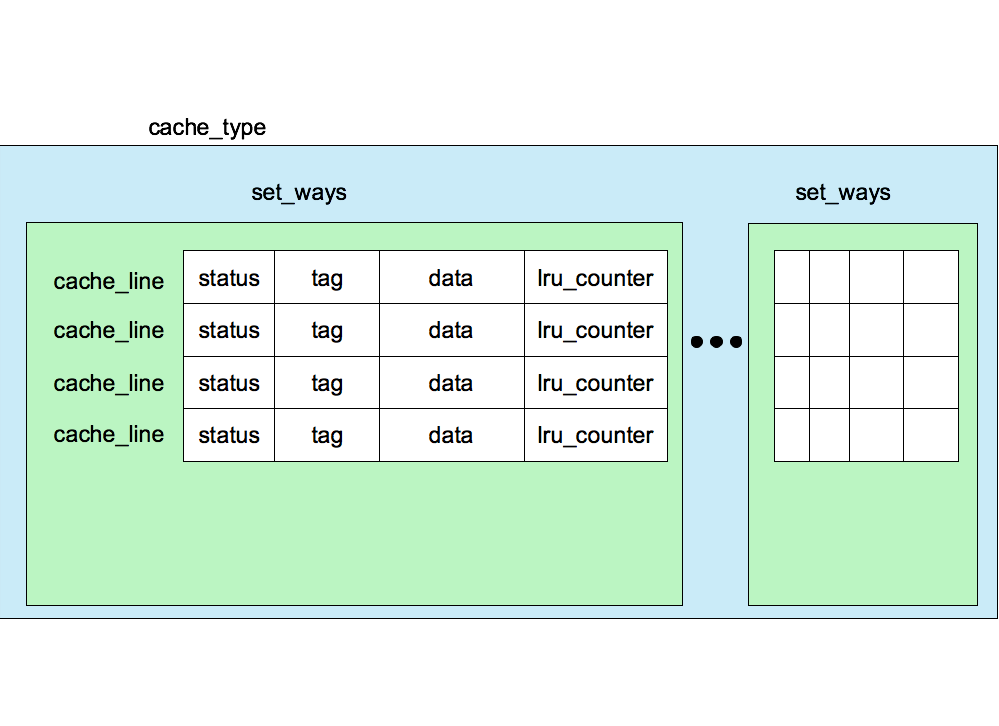
\includegraphics[width=\textwidth]{img/testbench/cacheType.png}
%\caption{Schematizzazione delle strutture dati della cache}
%\label{fig:c_type}
%\end{figure}
\subsection{Cache_test_snoop.vhd}

\section{Assembler per DLX}

Dopo avere testato individualmente il funzionamento dei componenti cache e RAM, si \`e passati al test del corretto funzionamento della cache inserita all'interno del progetto del processore DLX.\\
Per far ci\`o sono stati realizzati una serie di programmi in assembler, della quale mostreremo solo i due maggiormente significativi:
\begin{itemize}
 \item \texttt{provaReplacement123}: nel quale si verifica la corretta comunicazione tra cache e DLX e il meccanismo di rimpiazzamento.
 \item \texttt{provaFU}: nel quale si verifica il corretto funzionamento della Forwarding unit. 
\end{itemize}

\subsection{Dal codice all'escuzione}
Per completezza in questa sezione si spiegher\`a brevemente come poter mettere in esecuzione un codice assembler.
In primo luogo \`e necessario scrivere il codice in assembler all'interno di un file con estensione *.dls, che viene poi dato in pasto all'assemblatore DASM. Quest'ultimo lo converte in codice macchina mediante il seguente comando, eseguito dal prompt di comandi Windows:\\

\texttt{dasm -a -l <nome\_file>.dls}\\

Il risultato sar\`a un file \texttt{<nome\_file>.dlx} che a sua volta dovr\`a essere convertito mediante la classe java \texttt{DLXConv},eseguendo dal prompt di comandi Windows:

\texttt{java DLXConv <nome\_file>.dlx}\\

 per avere un file  \texttt{<nome\_file>.dlx.txt} contenente il codice in un formato direttamente inseribile all'interno del progetto del DLX.\\

In particolare quest'ultimo dovr\`a essere inserito nel file \texttt{Fetch\_Stage.vhd} all'interno dell'array che sostituisce la EPROM contenente le istruzioni in linguaggio macchina, da dare in pasto al processore:\\

\lstset{language=VHDL, caption=Inserimento del codice nella memoria istruzioni, label=DescriptiveLabel, breaklines=true, basicstyle=\small, showspaces=false, showtabs=false, stringstyle=\ttfamily, showstringspaces=false,  tabsize=3} % basicstyle=\tiny\ttfamily}

\begin{lstlisting}

constant EPROM_inst: eprom_type(0 to 11) := ( 
-- istruzioni in linguaggio macchina.
);

\end{lstlisting} 

\subsection{Codice assembler}
In questo paragrafo si analizzeranno nel dettaglio i codici assembler dei due test pi\`u significativi.
Per comodit\`a si riporter\`a il codice contenuto nella \texttt{EPROM\_inst} corredato di commento e codice assembler relativo.

 \subsubsection{provaReplacement123}
\lstset{language={[x86masm]Assembler}, caption=Codice assembler per il test del meccanismo di rimpiazzamento, label=DescriptiveLabel, breaklines=true, basicstyle=\footnotesize\ttfamily, showspaces=false, showtabs=false, showstringspaces=false,  tabsize=3} % basicstyle=\tiny\ttfamily}

\begin{lstlisting}
X"20010000",	--l1: addi r1,r0,0 ; azzera r1
X"20020001",	--l2: addi r2,r0,1 ; imposta a 1 r2
X"AC220000",	--l3: sw 0(r1),r2 ; memorizzza il valore di r2 all'indirizzo 0+r1(via 1 dell index0)
X"20420001",	--l4: addi r2,r2,1 ; incrementa r2
X"AC220100",	--l5: sw 16#100(r1),r2 ; memorizzza il valore di r2 all'indirizzo 16#100+r1(via 0 dell index0)
X"20420001",	--l6: addi r2,r2,1 ; incrementa r2
X"AC220080",	--l7: sw 16#80(r1),r2 ; memorizzza il valore di r2 all'indirizzo 16#80+r1(replacement via 1 dell index0) 
X"8C220000",	--l8: lw r2,0(r1) ; ripristina valore iniziale di r2 (1)
X"20210004",	--l9: addi r1,r1,4 ; incremento di 4 indirizzo di base in r1
X"0BFFFFE0",	--l10: j l3 ;
X"FFFFFFFF",	--NOP 
X"FFFFFFFF" 	--NOP

\end{lstlisting} 


\subsubsection{provaFU}

\lstset{language={[x86masm]Assembler}, caption=Codice assembler per il test della Forwarding Unit, label=DescriptiveLabel, breaklines=true, basicstyle=\footnotesize\ttfamily, showspaces=false, showtabs=false, showstringspaces=false,  tabsize=3} % basicstyle=\tiny\ttfamily}

\begin{lstlisting}
X"AC22000A",  --l1: sw 10(r1),r2  ; salva il contenuto di r2
X"8C23000A",  --l2: lw r3,10(r1)  ; porta in r3 il valore presente in r2
X"20620001",  --l3: addi r2,r3,1  ; incrementa r2
X"0BFFFFF0",  --l4: j l1          ; salta a l1
X"FFFFFFFF",
X"FFFFFFFF",

\end{lstlisting} 
